\documentclass[review]{elsarticle}
%-----------------------------------------------------

\usepackage{amsmath}
\usepackage{graphicx}

\graphicspath{{./figs/}}

\newcommand{\ihat}{\boldsymbol{\hat{\textbf{\i}}}}
\newcommand{\jhat}{\boldsymbol{\hat{\textbf{\j}}}}
\newcommand{\roughly}{{\raise.17ex\hbox{$\scriptstyle\sim$}}}
\newcommand{\dmax}{d_\text{max}}
\newcommand{\dmin}{d_\text{min}}

%-----------------------------------------------------

\makeatletter
\renewcommand{\fnum@figure}{Figure 2}
\makeatother

\thispagestyle{empty}

\begin{document}
\allowdisplaybreaks

\begin{figure}[ht]
\centering
%\includegraphics[width=\textwidth]{Figure_02_HR.pdf}
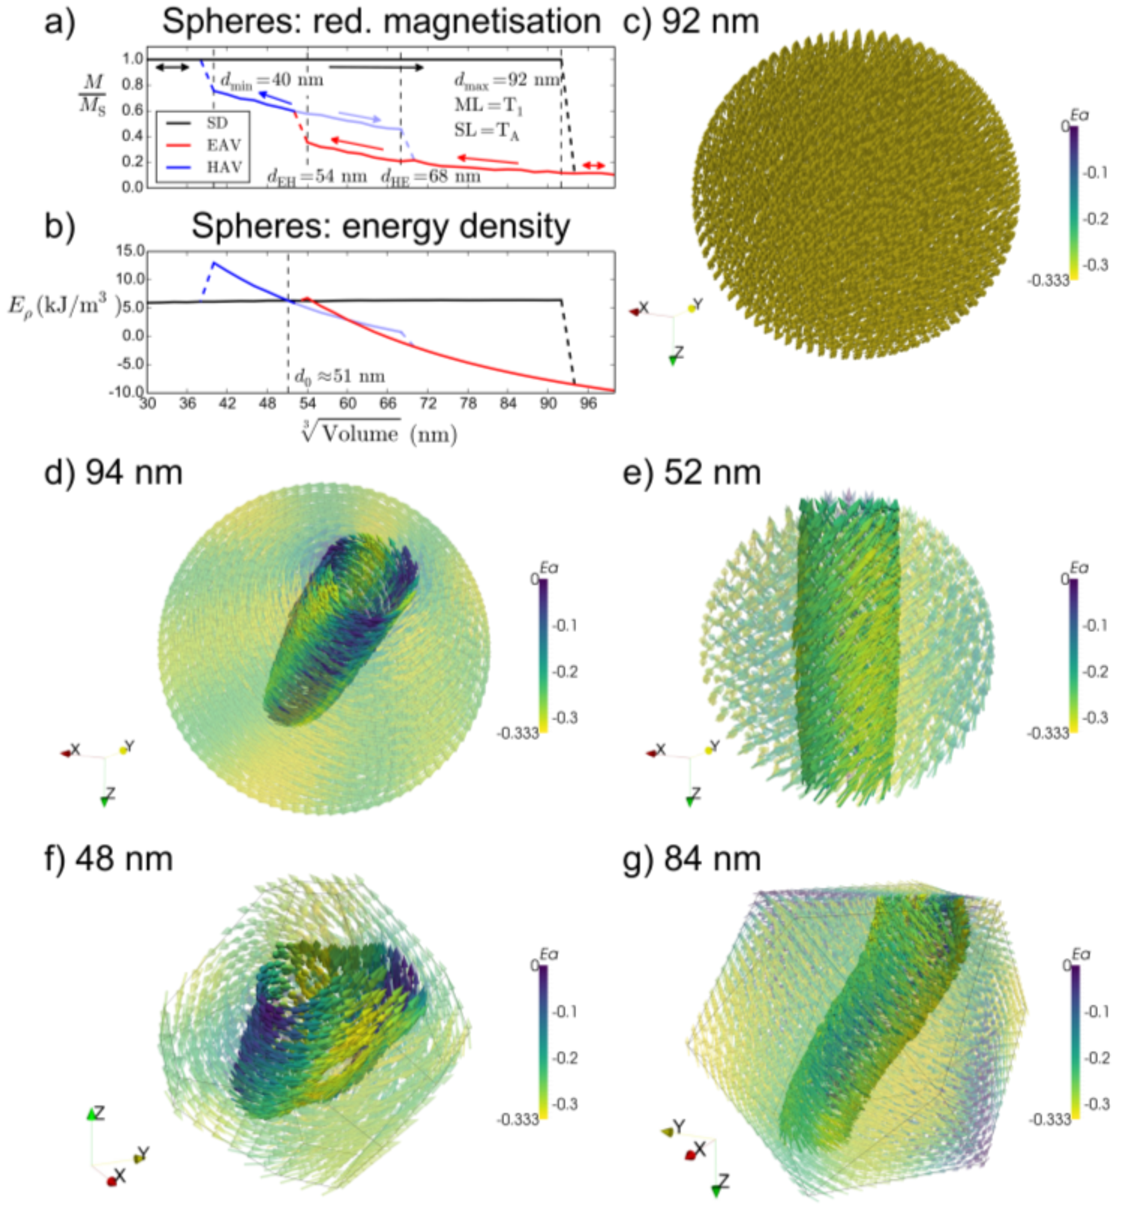
\includegraphics[width=\textwidth]{Figure_02.pdf}
\caption{Micromagnetic structures of spheres and intermediate-aligned vortex states. Reduced magnetisation (a) and energy density (b) against size. The SD [$\bar{1}\bar{1}\bar{1}$] state is numerically stable up to $\dmax=92\,\text{nm}$ (c). Growing this solution to a 94$\,\text{nm}$ grain it is found to relax to a [$\bar{1}\bar{1}\bar{1}$] EAV (d), stable up to 120$\,\text{nm}$. The EAV is then interpolated into smaller grains, stable down to $d_\text{EH}=54\,\text{nm}$ (a). At 52$\,\text{nm}$ the EAV goes to a [00$\bar{1}$] HAV (e), stable down to $\dmin=40\,\text{nm}$. At 38$\,\text{nm}$, the solution relaxes to the original SD state (a). This sequence is referred to as a Type 1 \textit{main loop} (ML). Growth of the HAV from 52$\,\text{nm}$ forms the Type A \textit{secondary loop} (SL): the HAV is found to be stable up to $d_{\text{HE}}=68\,\text{nm}$ (a) and to realign with the easy direction at 70$\,\text{nm}$. Vortex states can not only be easy or hard-aligned, but also $<$011$>$ intermediate-aligned vortices (IAVs) (f) and distorted IAV configurations (dIAV) (g). MLs in which IAVs are found are referred to as Type 2. Colour represents the MCA energy normalised by $|K_1|$. The vortex cores are highlighted by obtaining a helicity ($K=\boldsymbol{m}\cdot\nabla\times\boldsymbol{m}$) isosurface and reducing the opacity of the rest of the arrows.}
\label{fig2}
\end{figure}

\end{document}